% LTeX: enabled=true

\subsection{Important Notation}

To avoid ambiguity, we introduce the following notation conventions used throughout the paper.
For any $n \in \mathbb{N}$, we write $[n] \triangleq \{1, \ldots, n\}$  and $[n]_0 \triangleq [n] \cup \{0\}$. 
When using the notation $\bar{n}$, we refer to the unary representation of the number $n$; the plain symbol $n$
denotes the binary representation by default.
Given sets $A$ and $B$, we denote by $A^B \triangleq \{ f \mid f : A \to B \}$
the set of all functions from $B$ to $A$.
We define the Boolean domain as $\mathbb{B} \triangleq \{0, 1\}$,
the natural numbers as $\mathbb{N} \triangleq \mathbb{Z}_{\geq 1}$,
and the non-negative integers as $\mathbb{N}_0 \triangleq \mathbb{Z}_{\geq 0}$.


\subsection{Background overview}
As mentioned in the introduction, the current project works as an interaction
of three different fields: 1. counting complexity and combinatorial interpretation, 
2. total search problems and PPAD and 3. Kleene logic.


\subsubsection{Counting Complexity and Combinatorial Interpretations}
As we previously mentioned, we say that an object or a structure $f$
has a combinatorial interpretation if $f \in \textbf{\#P}$. $\textbf{\#P}$
is a complexity class created by Valiant \cite{valiant_ComplexityComputingPermanent_1979},
to define a formal combinatorial framework in complexity theory.


\begin{definitionbox}{$\textsc{\#P}$ Complexity Class}{sharpp-class}
    $\textbf{\#P}$ is a class of functions $f: \{0,1\}^* \to \mathbb{N}$
    such that: there
    exists a polynomial-time deterministic TM $M$, and
    $p : \mathbb{N} \to \mathbb{N}$ such that $p \in n^{O(1)}$, we have:
    $$
    f(w) = \Big|\Big\{v \in \{0,1\}^{p(|w|)} \mid M(w, v) =1 \Big\}\Big|
    $$
\end{definitionbox}

$\textbf{\#P}$ was initially created by \cite{valiant_ComplexityComputingPermanent_1979},
to demonstrate, that even if we have a problem $L \in P$, $\#L$ can be computationally
hard to compute, by providing an example of computing the permanent of
a 01-matrix, with number of perfect matchings. 

As we can see, $\textbf{\#P}$ allows us to define a set of objects,
whose cardinality equals $f(w)$. Core reasoning for choosing
$\textbf{\#P}$ to define combinatorial objects is mainly for the 
following two reasons \cite{ikenmeyer_PositivitySymmetricGroup_2024}: 

\begin{enumerate}
    \item By polynomially bounding words, we avoid cases such as: $f(w) = \{1, \hdots, f(w)\}$
    \item Current framework allows us to work with $f(\cdot)$, whose direct computation can be computationally hard
\end{enumerate}


The current framework was used in several papers such as
\cite{ikenmeyer_WhatWhatNot_2022} and \cite{ikenmeyer_PositivitySymmetricGroup_2024}
where they were able to use tools from complexity theory to show that
many structures do or do not have a combinatorial interpretation.
For the purposes of the current project, we are focusing on \cite{ikenmeyer_WhatWhatNot_2022},
where they demonstrated how several $\textsc{TFNP}$ problems, 
change in complexity as we ignore one of its solutions.


Any class of problems in complexity theory utilises the notion of reduction
to indicate the similarity between problems. For counting complexity
this is referred to as \textit{parsimonious reductions} \ref{def:pars-reduction}.


\begin{definitionbox}{Parsimonious reductions}{pars-reduction}
    Let $R, R'$ be search problems and let $M$ be a Karp reduction of
    $S_R = \{x \mid R(x) \neq \emptyset \}$ to $S_{R'} = \{x \mid R'(x) \neq \emptyset \}$.
    We say $f$ is \textbf{parsimonious} if:
    $$
    \forall x \in S_R : |R(x)| = |R'(f(x))|
    $$ 
\end{definitionbox}

\subsubsection{Total Search Problems and PPAD}
When talking about search problems, we are using the following definition:

\begin{definitionbox}{Search Problems and Total Search Problems}{search-problems}
    \textbf{Search problems} can be defined as relations $R \subseteq \{0,1\}^* \times \{0,1\}^*$,
    where given $x \in \{0,1\}^*$, we want to find $y \in \{0,1\}^*$  such that $x Ry$.

    \textbf{Total Search problems} are search problems such that:
    $$
    \forall x \in \{0,1\}^*, \exists y \in \{0,1\}^* : xRy
    $$
\end{definitionbox}

Using the above, we can define the following complexity classes

\begin{definitionbox}{$\scn{FNP}$ and $\scn{TFNP}$}{fnp-tfnp}
    \textbf{FNP} are \textit{search problems} such that there exists poly-time TM $M: \{0,1\}^* \to \{0,1\}$
    and a poly function $p : \mathbb{N} \to \mathbb{N}$ such that:
    $$
    \forall x \in \{0,1\}^*, y \in \{0,1\}^{p(|x|)}: xRy \iff M(x,y) = 1
    $$
    Lastly $\textbf{TFNP} = \{L \in \textbf{FNP} \mid L \text{ is total}\}$
\end{definitionbox}


\begin{definitionbox}{Levin Reductions}{levin-red}
    Given a pair of search problems $R_A, R_B$, a pair of
    computable time functions $(f,g)$ is called a Levin reduction from $R_A \to R_B$
    \begin{gather*}
        S_R \triangleq \{x \mid \exists y : xRy  \}\\
        R(x) \triangleq \{y \mid x Ry \} \\
        \forall x \in S_{R_A}, y_b \in R(f(x)):  (x , g(x, y_b)) \in R_A
    \end{gather*}
\end{definitionbox}


Levin reductions are the equivalent of \textit{Kerp reductions} for search
problems. Our current work focuses on a specific subclass of $\textbf{TFNP}$ problems
which is defined as follows:

\begin{definitionbox}{\textit{EndOfLine} problem \cite{papadimitriou_ComplexityParityArgument_1994}}{eol-ppad}
    Given circuits $S, P \in \{0,1\}^n \to \{0,1\}^n$ such that $S,P \in n^{O(1)}$
    we define a directed graph $G = (V,E)$, such that $V= \{0,1\}^n$ and $E$ defined as:
    $$
    E = \{(x,y) \in V^2: S(x) = y \wedge P(y) = x\}
    $$
    We define source or sinks $\forall v \in V: \textit{deg}(v) = (0,1)$ or
    $\textit{deg}(v) = (1,0)$, respectively. 
    We also syntactially ensure that the $0^n$ node is always a source, meaning
    $S(P(0^n) \neq 0 \wedge P(S(0^n)) = 0^n$.
    A node $v \in V$ is a solution if and only if $\textit{deg}(v)$ is either
    $(0,1)$  or $(1,0)$.
\end{definitionbox}


\begin{figure}[h!]
    \centering
    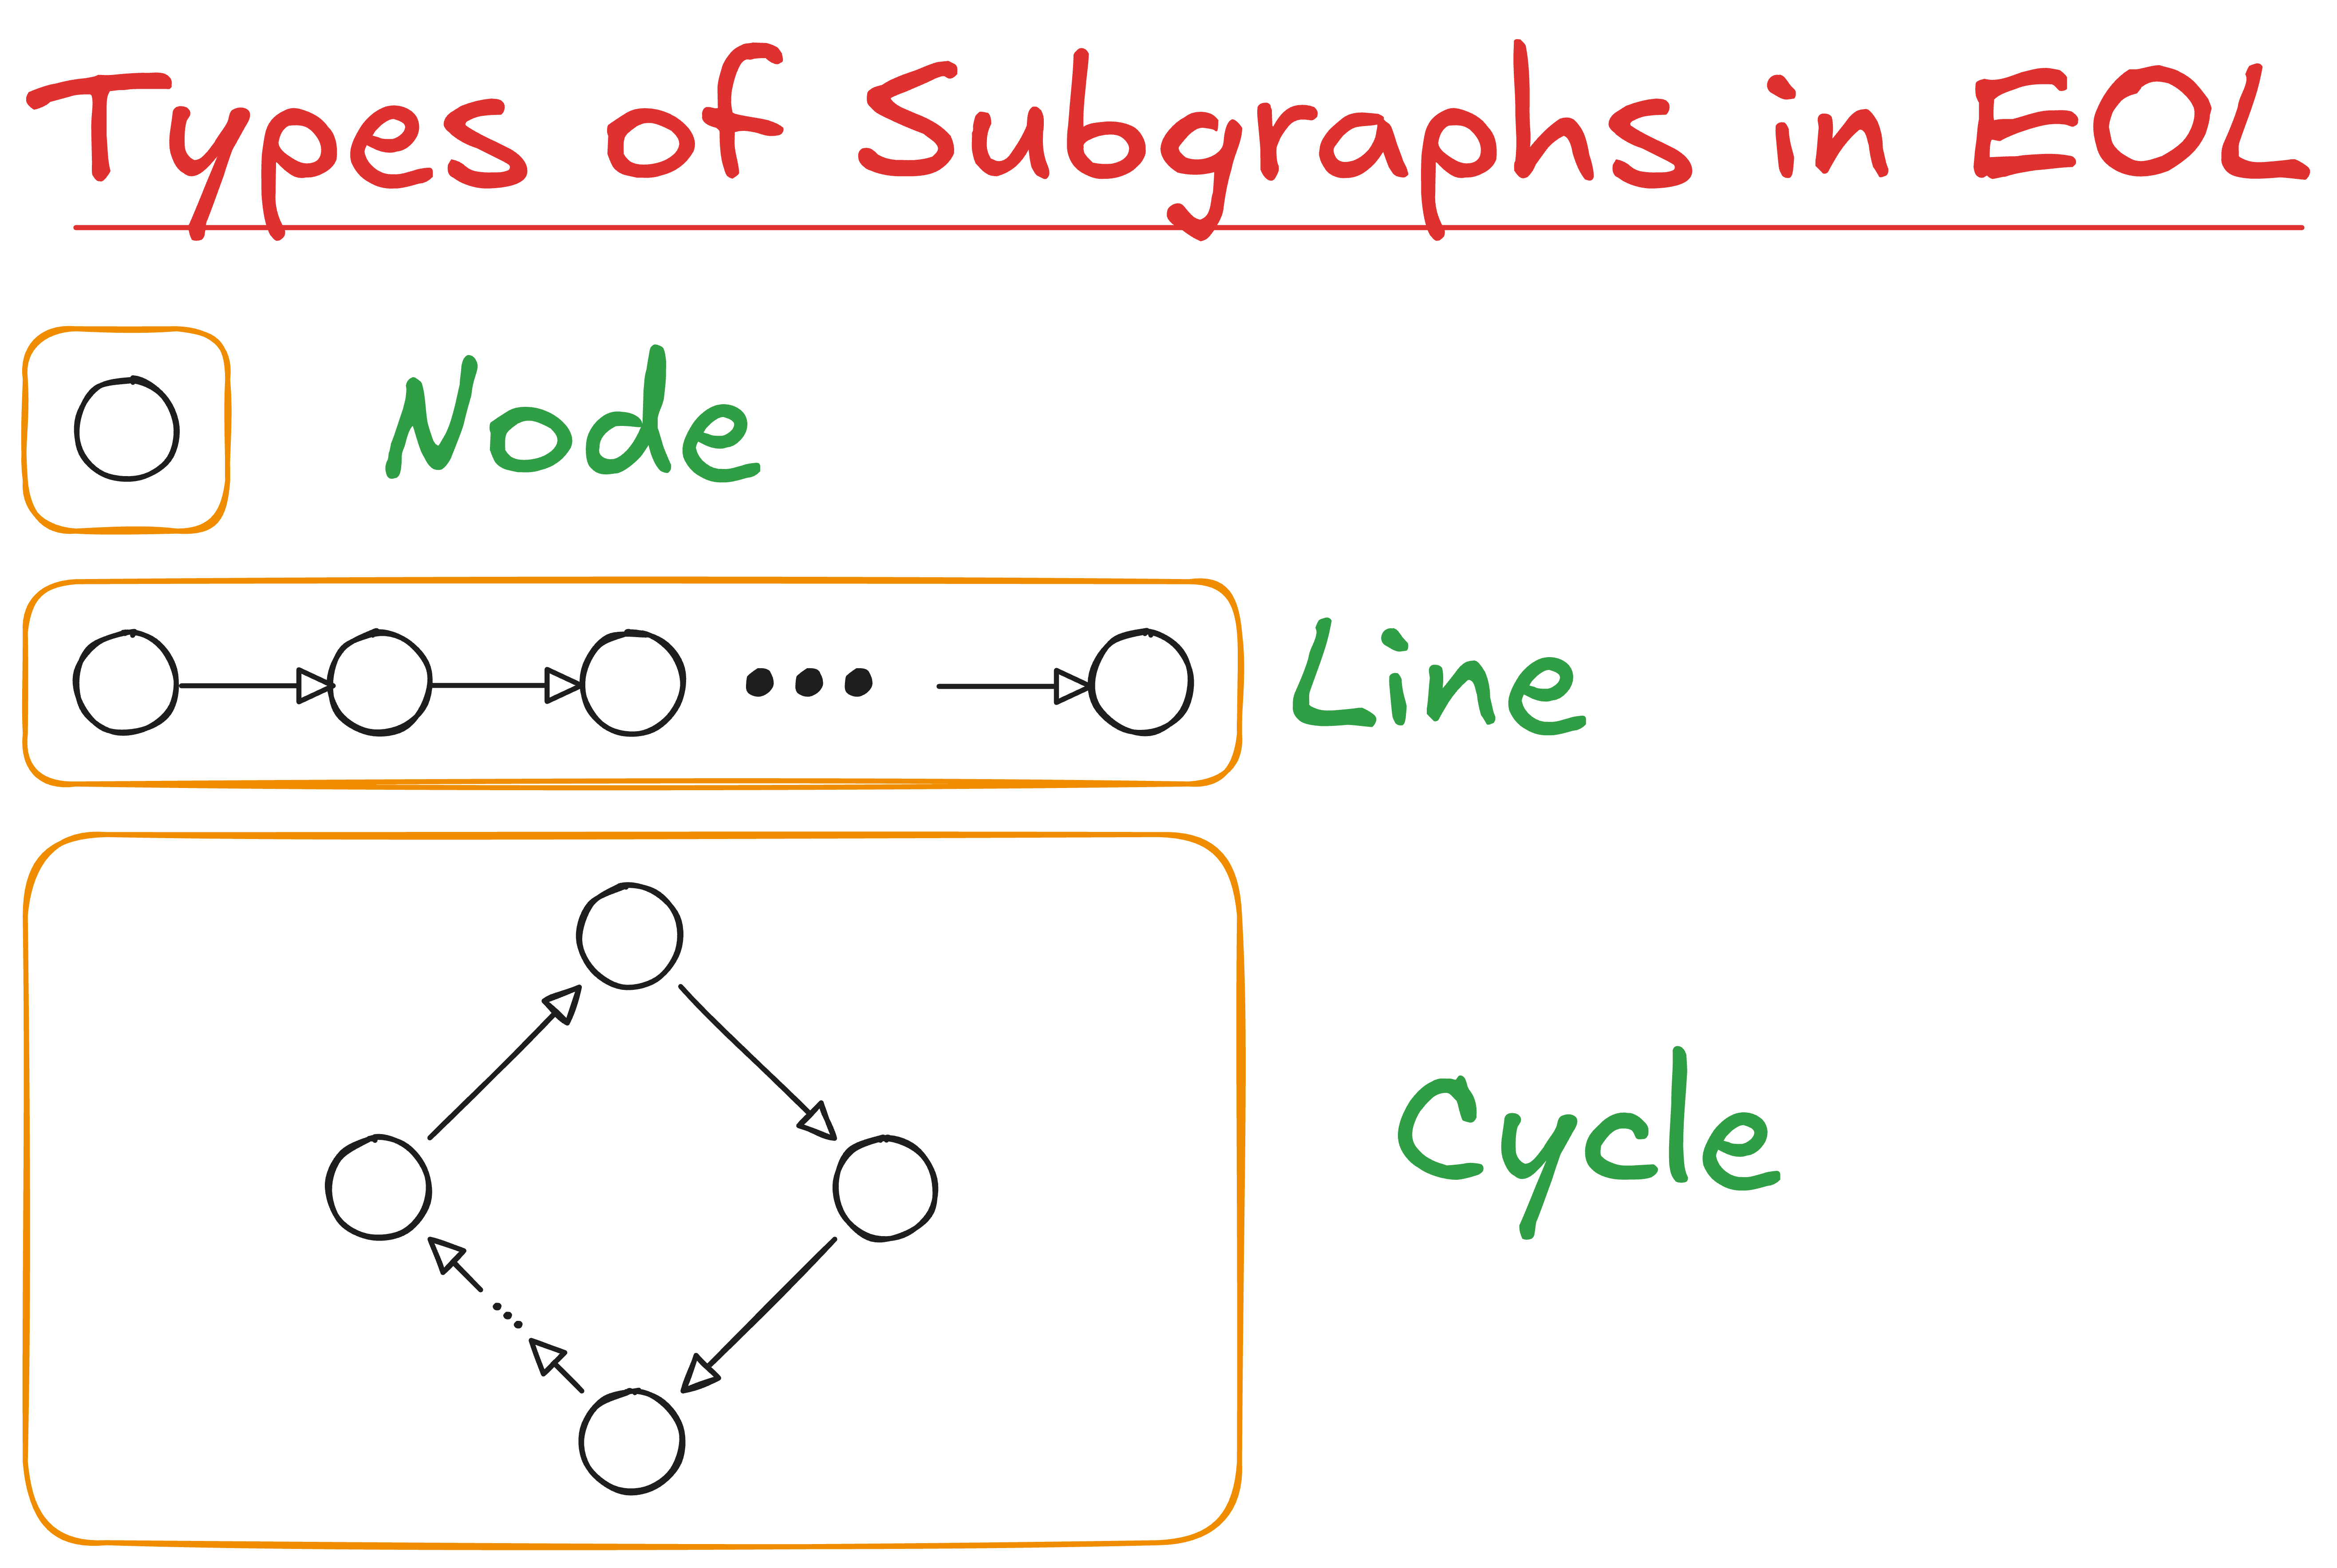
\includegraphics[width=0.3\textwidth]{assets/eol-subgraphs.png}
    \caption{Types of subgraphs in \textsc{EndOfLine}}\label{fig:eol-subgraphs}
\end{figure}


An illustrative example of an instance can be seen in the figure \ref{fig:eol-subgraphs}. A solution
to such problem instances are all the directed leafs and to ensure that a solution always
exists, we ensure that the $0^n$. Using the \textsc{EndOfLine} problem, we define the
\textsc{PPAD} complexity class \ref{def:ppad-complexity-class}


\begin{definitionbox}{\textsc{PPAD} complexity class \cite{papadimitriou_ComplexityParityArgument_1994}}{ppad-complexity-class}
    \textsc{PPAD} is defined as the set of search problems that
    are \textit{Levin reducible} \ref{def:levin-red} to the \scn{EndOfLine} problem \ref{def:eol-ppad}.
\end{definitionbox}

\textbf{PPAD} has been created by Papadimitriou \cite{papadimitriou_ComplexityParityArgument_1994}
to demonstrate a subset of problems in \textbf{NP} that are guaranteed to have
a solution but can be very difficult to find. In the next section
we will introduce the core set of \textsc{PPAD} problems that we are working with.

\paragraph{The PureCircuit problem}

Below we will introduce the
\textsc{PureCircuit}, which was create initially by
Deligkas et al. \cite{deligkas_PureCircuitTightInapproximability_2024}
to demonstrate the hardness of approximating \textsc{PPAD} problems.
This problem uses a kleene-logic based circuit construction with the help
of continuity of arguments, they demonstrated \textsc{PPAD-completeness}.

\begin{definitionbox}{\textsc{PureCiruit} Problem Definition \cite{deligkas_PureCircuitTightInapproximability_2024}}{purecircuit-def}
An instance of \textit{PureCircuit} is given by vertex set $V= [n]$ and gate set $G$ such that
$\forall g \in G: g=(T,u,v,w)$ where $u,v,w \in V$ and $T \in \{\text{NOR}, \text{Purify}\}$.
Each gate is interpreted as:
\begin{enumerate}
    \item \textit{NOR}: Takes as input $u,v$ and outputs $w$
    \item \textit{Purify}: Takes as input $u$ and outputs $v,w$
\end{enumerate}
And each vertex is ensured to have $\text{in-deg}(v) \leq 1$.
A solution to input instance $(V,G)$ is denoted as an assignment $\mathbf{x} : V \to \{0, \bot, 1\}$
such that for all nodes we have:
\begin{enumerate}
    \item if $v$ is the output of a $(\textit{NOR}, u,v,w)$ gate:
       \begin{gather*}
            \mathbf{x}[u] = \mathbf{x}[v] = 0 \implies \mathbf{x}[w] = 1\\
            (\mathbf{x}[u] =1 \vee \mathbf{x}[v] =1) \implies \mathbf{x}[w] = 0 \\
            \text{otherwise} \implies \bot
        \end{gather*}

    \item \textit{Purify}: 
       \begin{gather*}
           \forall b \in \{0,1\}: \mathbf{x}[u] = b \implies \mathbf{x}[v] = b \wedge \mathbf{x}[w] =  b\\
           \mathbf{x}[u] = \bot \implies \{\mathbf{x}[v] \cup \mathbf{x}[w] \} \cap \{0,1\} \neq \emptyset
        \end{gather*}
\end{enumerate}
\end{definitionbox}

The definition of \textsc{PureCircuit} that we will be using for the standard set of gates
$\{\wedge, \vee, \neg\}$, is based Kleene's three-valued strong logic of indeterminancy
which extends the traditional $\mathbb{B}$ logic \cite{kleene_IntroductionMetamathematics_2009}.
In addition to that, we will make use of the \textit{Copy} gate but adding the robustness
constraint such that if $(\textit{Copy},u,v) \in G \implies x[u] = x[v]$.
This allows our circuits to be robust and easier to work with.



For the \textit{Purify} gate,
Deligkas et al. showed that the only solutions that are essential for \textit{Purify}
are $\{(0,\bot), (\bot,1), (0,1)\}$ with the help of continuity arguments \cite{deligkas_PureCircuitTightInapproximability_2024}.
Adding more solutions does not change the complexity as he showed in the original variant of the problem.
We acknowledge that the solution set will be different than the original one but
we can easily observe that  $\textsc{\#PureCircuit-simplified} \subseteq \textsc{\#PureCircuit}$,
and therefore any proposition or argument of the sort: $\textsc{\#A} \subseteq \textsc{\#PureCircuit-simplified}$
still holds true. For the purposes of the report, any solution change will be made explicit
and we will refer to all such simplified variants as $\textsc{\#PureCircuit}$ to avoid
confusion. 



\begin{definitionbox}{\textsc{SourceOrExcess} problem}{source-or-excess}
    We define as $\textit{SourceOrExcess}(k,1)$ for $k \in \mathbb{N}_{\geq 2}$
    the search problem as such: Given a poly-sized successor circuit $S : \{0,1\}^n$
    and a set of predecssor poly-sized circuits $\{P_i\}_{i \in [k]}$, we define
    the graph $G = (V,E)$ such that, $V = \{0,1\}^n$ and $E$ as:
    $$
    \forall x, y \in V: (x,y) \in E \iff (S(x) = y) \wedge \bigvee_{i \in [k]} P_i(y) = x
    $$
    We ensure that $0^n$ is as sink, meaning $\text{deg}(0^n) = (0,1)$.
    A valid solution is a vertex $v$ such that $\textit{in-deg}(v) \neq \textit{out-deg}(v)$
\end{definitionbox}

\paragraph{Sperner problems}

Below we will refer to the notion of Sperner problems which involve
the idea of using the topology of a problem and a colouring scheme to ensure
that a substructure is panchromatic. There two variants of colouring scheme
that are used: one of them will be referred to as the \textbf{linear} colouring
where for dimension $d$, assign $d+1$ distinct colours to each point \cite{daskalakis_ComplexityComputingNash_2006, chen_Complexity2DDiscrete_2009}.
Below we will refer to \textbf{bipolar} colouring, which has been used grid-like topologies of the Sperner property
\cite{chen_SettlingComplexityComputing_2009, deligkas_PureCircuitTightInapproximability_2024, daskalakis_ComplexityConstrainedMinmax_2021}.
It has to be noted that these are not their official names, but we have decided
to use this naming scheme for clarity.



\begin{definitionbox}{Bipolar colouring}{bipolar-colouring}
    Given dimension $d$, we refer to the bipolar colouring $C$ of a point $v \in S^d$
    where $S$ is some arbitrary set in $d$ dimensionality the following:
    $$
    \forall j \in [d]: [C(v)]_j \in \{-1,1\}
    $$
    Essentially a point is a associate with a $d$ dimensionaly binary vector.
    We say that a set of points $A \subseteq S^d$ \textbf{cover all the labels} if:
    $$
        \forall i \in [d], \ell \in \{-1, +1\}, \exists x \in A: [\lambda(x)]_{i} = \ell
    $$
\end{definitionbox}



\begin{definitionbox}{\textsc{StrongSperner} problem}{strong-sperner}
    \textbf{Input}: A boolean circuit that computes a bipolar labelling $\lambda: [M]^N \to \{-1, 1\}^N$ \ref{def:bipolar-colouring}
    satisfying the following boundary conditions $\forall i \in [N]$:
    \begin{itemize}
        \item if $x_i = 1 \implies [\lambda(x)]_i = +1$
        \item if $x_i = M \implies [\lambda(x)]_i = -1$
    \end{itemize}
    \textbf{Output}: A set of points $\{x^{(i)}\}_{i \in [N]} \subseteq [M]^{[N]}$, such that:
    \begin{itemize}
        \item \textit{Closessness condition}: $\forall i,j \in [N]: \|x^{(i)} - x^{(j)}\|_{\infty} \leq 1$
        \item \textit{Covers all labels} as defined in \ref{def:bipolar-colouring}
    \end{itemize}
\end{definitionbox}

The above is a generalised variant of the tradtional Sperner problem to
a grid of dimensions $N$ and width of $M$. 
Throughout literature the same variants of the problem or specifications
have been defined using sperner or discrete brouwer \cite{chen_SettlingComplexityComputing_2009, chen_Complexity2DDiscrete_2009, daskalakis_ComplexityComputingNash_2006, deligkas_PureCircuitTightInapproximability_2024}.
For the sake of clarity, we will stick to $\textsc{StrongSperner}$.

\begin{definitionbox}{$\scn{nD-StrongSperner}$ problem}{nd-strong-sperner}
    \textbf{Input}: A tuple $(\lambda,0^k)$ of a $\scn{StrongSperner}$ instance but for only $n$ dimensions, such that
    $\lambda : (\{0,1\}^k)^n \to \{-1, +1\}^n$.\\
    \textbf{Output}: A point $\alpha = (a_1, \hdots, a_n) \in A^n$, where $A=\{0,1\}^k \setminus \{1^k\}$ such that:
    $$
    \{\alpha + x \mid x \in \{0,1\}^n\} \text{ cover all the labels \ref{def:bipolar-colouring}}
    $$
    We use $A$ to avoid edge cases. We assume dimensionality $n \geq 2$.
\end{definitionbox}

Chen et al. \cite{chen_SettlingComplexityComputing_2009} demonstrated 
that all $\textsc{nD-StrongSperner}$ are $\textsc{PPAD-complete}$.
We mainly use this to show counting arguments with respect to the
\textsc{EndOfLine} as people have indicated a parsimonious reduction
between $\textsc{2D-StrongSperner}$ 
and $\textsc{3D-StrongSperner}$ to the EndOfLine problem but 
with \textit{linear} colouring. The authors of these papers
use these problems indifferently when talking about the reductions
and therefore we can assume that either colouring will create a correct reduction.

\paragraph{Other PPAD problems}





\pargraph{Counting complexity of PPAD}

These problems have found
connections with various other problems such as Nash Equilbria,
Fixed point theorems or Sperner Lemmas. The current project looks
on the counting complexity of such problems as despite two problems
being PPAD-complete, Ikenmeyer et al. \cite{pak_WhatCombinatorialInterpretation_2022} has showed several examples where
their counting difficulty can differ vastly. Examples of such statements
can be summarised as:

\begin{gather*}
    \textbf{\#PPAD}(\textsc{SourceOrSink})-1/2  = \textbf{\#P}\\
    \textbf{\#P}^A \not\subseteq \textbf{\#PPAD}(\textsc{SourceOrExcess(2,1)})^A-1
\end{gather*} 


Currently we are mainly focused into the study of a certain 
$\textbf{PPAD}\textit{-complete}$ problem, known as $\textsc{PureCircuit}$

\subsubsection{Kleene Logic and Hazard-Free Circuits}

Kleene logic, is the type of system that extends the traditional %% Please triple check it just in case you get nuked for this
binary system to: $\mathbb{T} = \{0, \bot,1 \}$. 
Study of such systems has an impact to both
the development of robust systems and from a theoritical point of view,
people developed systems such as \textit{Alternative Turing mahcines}, as well as
showing important correlations between the complexity of monotone circuits
and the robustness of hazard free circuits. 

We want to introduce the following concepts:

\begin{definition}[Kleene Resolutions]
    Given $x \in \mathbb{T}^n$, we define the \textit{resolutions} of $x$, using the following notation:
    $$
    \scn{Res}(x) \triangleq \big\{ y \in \mathbb{B}^n \mid \forall j \in [n]: x_i \in \mathbb{B} \implies x_i = y_i \big\}
    $$
\end{definition}

\begin{definition}[Hazard circuit]
    A \textit{circuit} $C$, on $n$ inputs has \textbf{hazard} at $x \in \mathbb{T}^n \iff C(x) = \bot$
    and $\exists b \in \mathbb{B}, \forall r \in \scn{Res}(x): C(r) = b$
\end{definition}


\begin{definition}[Natural function]
    A function $F: \mathbb{T}^n \to \mathbb{T}$ can be computed by stable values and is monotone with respect to $\preceq$
\end{definition}

\begin{definition}[K-bit Hazard]
    For $k \in \mathbb{N}$ at $x \in \mathbb{T}^n \iff C$  has a \textit{hazard} at $x$ and $\bot$ appears at most $k$ times in $x$
\end{definition}



